% Q1V3: Toroid with Cut (Air Gap) — Exam diagram (hybrid style C)
% Adapted from weekly/week10/diagrams/q3_toroid_physical.tex
% Strips: B-field arrows, mu_r annotation on core (P-STACK-31)
% Keeps: core geometry, coil positions, gap, dimensions
\documentclass[border=10pt]{standalone}
\usepackage{tikz}
\usepackage{amsmath}
\usetikzlibrary{decorations.pathreplacing}
\renewcommand{\familydefault}{\sfdefault}

\begin{document}
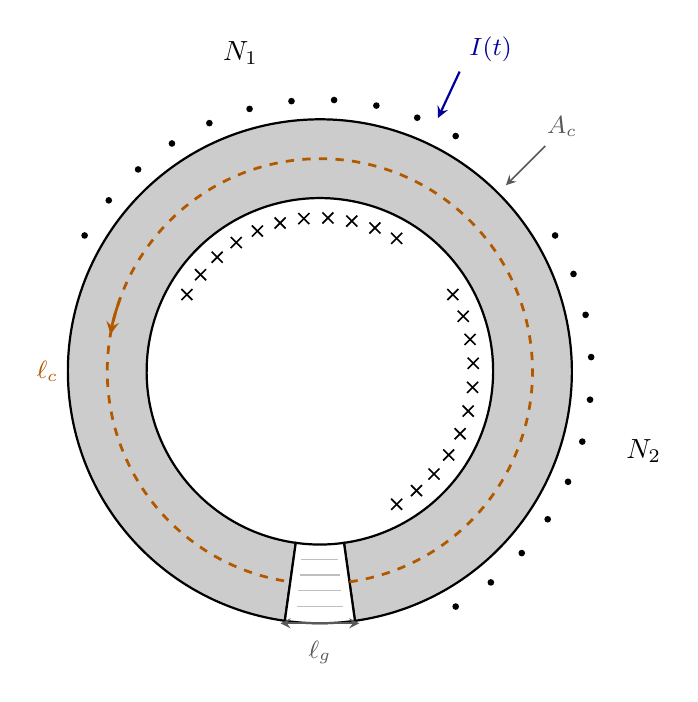
\begin{tikzpicture}[
    every node/.style={font=\sffamily},
    >=stealth,
    dim/.style={<->, line width=0.6pt, gray!70!black},
    dimlabel/.style={font=\sffamily\small, text=gray!70!black},
]

% Parameters
\def\Router{3.2}
\def\Rinner{2.2}
\def\Rmid{2.7}
\def\gapangle{8}  % half-angle of air gap (degrees)

% === Ferromagnetic core (annular arc, excluding gap at bottom) ===
\fill[gray!40, draw=black, line width=0.8pt]
    ({-90+\gapangle}:\Router) arc ({-90+\gapangle}:{270-\gapangle}:\Router)
    -- ({270-\gapangle}:\Rinner) arc ({270-\gapangle}:{-90+\gapangle}:\Rinner)
    -- cycle;

% === Air gap region (white with hatching) ===
\fill[white, draw=black, line width=0.8pt]
    ({-90-\gapangle}:\Router) arc ({-90-\gapangle}:{-90+\gapangle}:\Router)
    -- ({-90+\gapangle}:\Rinner) arc ({-90+\gapangle}:{-90-\gapangle}:\Rinner)
    -- cycle;

% Air gap hatching lines
\foreach \frac in {0.2, 0.4, 0.6, 0.8} {
    \pgfmathsetmacro{\r}{\Rinner + \frac*(\Router-\Rinner)}
    \draw[thin, gray!50] ({-90-\gapangle*0.7}:\r) -- ({-90+\gapangle*0.7}:\r);
}

% === Coil 1 windings (upper-left, 60-150 degrees) ===
\foreach \angle in {60,69,...,150} {
    % Outer winding: dot (current out of page)
    \fill ({(\Router+0.25)*cos(\angle)},{(\Router+0.25)*sin(\angle)}) circle (1.2pt);
    % Inner winding: cross (current into page)
    \pgfmathsetmacro{\xw}{(\Rinner-0.25)*cos(\angle)}
    \pgfmathsetmacro{\yw}{(\Rinner-0.25)*sin(\angle)}
    \draw[line width=0.6pt] ({\xw-0.07},{\yw-0.07}) -- ({\xw+0.07},{\yw+0.07});
    \draw[line width=0.6pt] ({\xw-0.07},{\yw+0.07}) -- ({\xw+0.07},{\yw-0.07});
}
\node[above] at ({(\Router+0.7)*cos(105)},{(\Router+0.7)*sin(105)}) {$N_1$};

% === Coil 2 windings (upper-right, 30-(-30) mapped to right side) ===
\foreach \angle in {-60,-51,...,30} {
    % Outer winding: dot
    \fill ({(\Router+0.25)*cos(\angle)},{(\Router+0.25)*sin(\angle)}) circle (1.2pt);
    % Inner winding: cross
    \pgfmathsetmacro{\xw}{(\Rinner-0.25)*cos(\angle)}
    \pgfmathsetmacro{\yw}{(\Rinner-0.25)*sin(\angle)}
    \draw[line width=0.6pt] ({\xw-0.07},{\yw-0.07}) -- ({\xw+0.07},{\yw+0.07});
    \draw[line width=0.6pt] ({\xw-0.07},{\yw+0.07}) -- ({\xw+0.07},{\yw-0.07});
}
\node[right] at ({(\Router+0.7)*cos(-15)},{(\Router+0.7)*sin(-15)}) {$N_2$};

% === Dimension: air gap length ===
\draw[dim] ({-0.5},{-\Rmid-0.5}) -- ({0.5},{-\Rmid-0.5});
\node[dimlabel, below] at (0,{-\Rmid-0.6}) {$\ell_g$};

% === Dimension: cross-sectional area ===
\draw[->, line width=0.6pt, gray!70!black]
    ({(\Router)*cos(45)+0.6},{(\Router)*sin(45)+0.6})
    -- ({(\Router)*cos(45)+0.1},{(\Router)*sin(45)+0.1});
\node[dimlabel, above right] at ({(\Router)*cos(45)+0.5},{(\Router)*sin(45)+0.6}) {$A_c$};

% === Mean magnetic path (dashed circle at mean radius, excluding gap) ===
\draw[dashed, line width=1.0pt, orange!70!black]
    ({-90+\gapangle}:\Rmid) arc ({-90+\gapangle}:{270-\gapangle}:\Rmid);
\node[dimlabel, left, text=orange!70!black] at ({180}:{\Rmid+0.5}) {$\ell_c$};
% Arrow indicator on the path
\draw[->, orange!70!black, line width=1.0pt]
    ({160}:\Rmid) arc ({160}:{170}:\Rmid);

% === Current arrow on primary ===
\draw[->, thick, blue!60!black]
    ({(\Router+1.0)*cos(65)},{(\Router+1.0)*sin(65)})
    -- ({(\Router+0.35)*cos(65)},{(\Router+0.35)*sin(65)});
\node[above right, font=\sffamily\small, text=blue!60!black]
    at ({(\Router+1.0)*cos(65)},{(\Router+1.0)*sin(65)}) {$I(t)$};

\end{tikzpicture}
\end{document}
